\documentclass[a4paper,twoside,12pt,AutoFakeBold]{ctexart}
\newcommand\specialsectioning{\setcounter{secnumdepth}{-2}}
\specialsectioning
\usepackage[center]{titlesec}
\usepackage{indentfirst}
\setlength{\parindent}{2em}
\usepackage{fancyhdr}
\pagestyle{fancy}%fancy style
\usepackage{caption}
\fancyhf{}%清空页眉页脚
\fancyhead[LE,RO]{\thepage}%页码位置:偶数页居左,奇数页居右
\fancyfoot[RO,RE]{\textit{NEFU's seminar of Marxism}}% 设置页脚:在每页的右下脚以斜体显示书名
\usepackage{graphicx}
\setlength{\headheight}{15pt}%解决页眉warnings
\usepackage{amsmath}
\renewcommand{\headrulewidth}{0pt} % 页眉与正文之间的水平线粗细
\renewcommand{\footrulewidth}{0pt}
\usepackage{tcolorbox}%文本框宏包
\usepackage{changepage}%设置引用段落左右侧缩进

\usepackage{tabularx}
\usepackage{hyperref}%设置超链接
\usepackage{float}
\title{读书会记录}
\author{东北林业大学马克思主义研讨会\\
指导教师:李光玉~许婕\\
 吴云飞~编}
\date{2023-11}
\usepackage{perpage}
\MakePerPage{footnote}
\begin{document}
\maketitle
\newpage



\tableofcontents%目录

\newpage

\section{序言}

\begin{adjustwidth}{2em}{2em}
\qquad\fangsong 
本书是东北林业大学马克思主义经典著作研究与讨论会的一个内部记录,诸多观点与看法可能会欠缺专业性,因而这是一个非教学性质的内容记录。本书全部内容均来自我们的研讨会中的发言与讨论以及后续编者所进行的思考,如有雷同,纯属巧合,本书最终解释权归本研讨会与编辑组\footnote{编者注:虽然称作是“编辑组”,但目前全组就我一个人,若是有擅长\LaTeX{}编译的并且有意愿加入本书编辑组的成员可以与我联系。}所有。

本书的\LaTeX{}源代码已由编者吴云飞托管至其本人的Github仓库之中,供各位成员获取:\url{https://github.com/Imheaven233/Seminar-of-Marxism-of-NEFU}。

\end{adjustwidth}




\newpage

\section{第一期:《哲学的贫困》选读(1)}

\subsection{学习提示}\label{sec:1}

《哲学的贫困》是马克思针对蒲鲁东的《贫困的哲学》一书而写的一部论战性著作,以法文写成于1847年上半年,并于同年7月在布鲁塞尔和巴黎出版。

该著作分为两个部分,即第一章和第二章。第一章的讨论针对蒲鲁东为“工资平等”的社会主义所作的经济学论证,揭示这种论证尚未达到李嘉图经济学理论的水准。第二章批判了蒲鲁东经济学理论的哲学基础。

本期讨论会我们选的内容是第二章“\textbf{政治经济学的形而上学}”的第一节“\textbf{方法}”,这部分内容在我们编排的讲义中的3—17页\footnote{编者注:这部分内容收录于马恩选集第1卷。}。

在本次讨论会中,您将会了解到(或带着以下问题去阅读):

\textbf{1.}马克思对黑格尔的辩证法的一个简要概述。

\textbf{2.}蒲鲁东的经济学理论所遵循的“辩证法”同黑格尔的辩证法之间的差异。

\textbf{3.}蒲鲁东的经济学理论的哲学基础之实质是什么,犯了什么错误?

\textbf{4.}对蒲鲁东的经济学理论的哲学基础的批判对于我们有何启示?

\subsection{读书会记录}
2023年10月16日18:00—20:00,我们在东北林业大学奥林学院203教室开展了第一期的读书会。本期读书会我们阅读了《哲学的贫困》第二章第一节的部分内容(截止到“\textbf{第五个说明}”之前),并做了充分的讨论。具体讨论内容可简要地概括如下:

\subsubsection{1.前言部分}\label{sec:3}

首先,马克思在前言部分指出:
\begin{adjustwidth}{2em}{2em}
\qquad\fangsong
“如果说有一个英国人把人变成帽子,那末,有一个德国人就把帽子变成观念。这个英国人就是李嘉图,一位银行巨子,杰出的经济学家;这个德国人就是黑格尔,柏林大学的一位专任哲学教授。”
\end{adjustwidth}

这段话中的“帽子”、“观念”指的是什么?在这里我们认为,“帽子”指的是李嘉图的经济学中的诸多“经济范畴”,体现着物与物之间的关系;而“观念”则指的是黑格尔哲学中的“概念”,更确切地说,是黑格尔哲学中的形而上学传统\footnote{这在后面的讨论中会详细的说明。}。

古典经济学家们\footnote{这里指的是英国古典经济学家斯密、李嘉图等人。}通过对资本主义社会的外部经验现象的考察总结出了一些基本的经济规律,但是他没有意识到这些规律本身并非是永恒不变的存在物,以至于他们将人与人之间关系转变为物与物之间的关系,企图通过不变的经济范畴(帽子)解释人类社会的运行本身\footnote{按照马克思的话就是:“把人变成帽子。”}。而持有着形而上学传统的哲学家们(尤指黑格尔)则将这些“帽子”进行了更进一步的“抽象”,将其转化为观念本身\footnote{按照马克思的话就是:“把帽子变成观念。”}。

\subsubsection{2.第一个说明}

第一个说明所讨论的核心内容是黑格尔的辩证法,而黑格尔的辩证法在整体上也是建筑于形而上学这一传统的基础之上的。马克思指出,经济学家们只是向我们解释了生产如何在现存的关系下进行,但是没有向我们解释这些“关系”本身是何以存在的。古典经济学家们面对的是活生生的现实,他们所做的工作是对“活生生的现实”的直接抽象;而蒲鲁东面对的则是古典经济学家们提出的诸多范畴,以及隐藏在这些范畴背后的诸多古典经济学家们的教条与偏见,蒲鲁东在探寻这些“关系”得以产生的原因的过程中,他仅仅从这些范畴本身出发,因而他只能在观念的领域兜圈子。

黑格尔哲学的第一步便是形而上学式的抽象,将一切事物都抽象成为逻辑范畴,并将一切事物的运动也抽象成纯粹形式的运动,这样一来,正如马克思所言:

\begin{adjustwidth}{2em}{2em}
    \qquad\fangsong
    “既然把任何一种事物都归结为逻辑范畴,任何一个运动、任何一种生产行为都归结为方法,那末,由此自然得出一个结论,产品和生产、对象和运动的任何总和都可以归结为应用的形而上学。黑格尔为宗教、法等做过的事情,蒲鲁东先生也想在政治经济学上如法炮制。”
\end{adjustwidth}

由此,黑格尔找到了一种“绝对的方法”来描绘现实世界的运动,即纯粹理性的运动。事实上,这是一种颠倒,但在这里我们就不赘述了\footnote{唯心主义与唯物主义之间的颠倒。}。在这里不难理解,当事物的一切“偶性”都被抽掉之后,剩下的就是纯粹的“概念”、纯粹的“理性”,但需要指出的是,这种纯粹的“概念”与“理性”是脱离个别主体而存在的,是一种绝对的、客观的东西。因此,对于黑格尔的辩证法而言,辨证运动是“绝对精神”的自我运动,是“概念”的自我规定,因而这是一种客观的唯心主义。


\subsubsection{3.第二个说明}

在这部分内容中的末尾,马克思表明了他的历史唯物主义哲学思想:

\begin{adjustwidth}{2em}{2em}
    \qquad\fangsong
    “经济学家蒲鲁东先生非常明白,人们是在一定的生产关系范围内制造呢绒、麻布和丝织品的。但是他不明白,这些一定的社会关系同麻布、亚麻等一样,也是人们生产出来的。社会关系和生产力密切相联。随着新生产力的获得,人们改变自己的生产方式,随着生产方式即保证自己生活的方式的改变,人们也就会改变自己的一切社会关系。手工磨产生的是封建主为首的社会,蒸汽磨产生的是工业资本家为首的社会。”
\end{adjustwidth}

事实上,上面这段话的第一句可以转译为:

\begin{adjustwidth}{2em}{2em}
    \qquad\fangsong
    蒲鲁东明白,人们在一定的“关系”内制造“物”。但是他不明白,这些“关系”同这些“物”一样,也是人们生产出来的。
\end{adjustwidth}
这充分说明了马克思的历史唯物主义哲学与那种纯粹被动的、毫无生机的机械唯物主义哲学之间的差异,因为马克思告诉我们,“关系”可不是什么神秘主义式的东西,“关系”本身就是通过人类的实践活动所建构出来的。

\subsubsection{4.第三个说明}

在“第三个说明”中,马克思揭示了蒲鲁东经济理论的矛盾。马克思是这么说的:

\begin{adjustwidth}{2em}{2em}
    \qquad\fangsong
    “每一个社会中的生产关系都形成一个统一的整体。蒲鲁东先生把种种经济关系看做同等数量的社会阶段,认为这些阶段一个产生一个,一个来自一个,正如反题来自正题一样;认为这些阶段在自己的逻辑顺序中实现着人类的无人身的理性。

这个方法的唯一短处就是:蒲鲁东先生在考察其中任何一个阶段时,都不能不靠其它一些社会关系来说明,可是当时这些社会关系尚未被他用辩证运动产生出来。当蒲鲁东先生后来借助纯粹理性使其它阶段产生出来时,却又把它们当成初生的婴儿,忘记它们和第一个阶段是同样年老了。

因此,要构成被他看做一切经济发展基础的价值,就非有分工、竞争等等不可。然而当时这些关系在一定的系列中、在蒲鲁东先生的理性中以及逻辑顺序中根本还不存在。”
\end{adjustwidth}
在这里可以看到,蒲鲁东的“辩证法”很有意思,当他运用“辩证法”推出某些新的概念时,他总是需要依靠一些尚未被他的“辩证法”所生成出来的东西去说明。例如,蒲鲁东通过A和B推出了C,再通过C和I推出了D,但是I本身并没有通过他的辩证法被创造出来,而当他通过E和F推出I的时候,他也忘记了,I本身在C到D的“辩证运动”中就已经作为前提条件生成了。因此,马克思在这里隐约地想表明,蒲鲁东的“辩证法”似乎是一种非辩证的主观臆想。

\subsubsection{5.第四个说明}

通过对前面部分的阅读与讨论,“第四个说明”这部分内容便显得容易理解了。马克思在这一部分中说明了蒲鲁东是如何将他的“辩证法”应用到政治经济学领域的。马克思是这么叙述的:

\begin{adjustwidth}{2em}{2em}
    \qquad\fangsong
“蒲鲁东先生认为,任何经济范畴都有好坏两个方面。他看范畴就象小资产者看历史伟人一样:拿破仑是一个大人物;他行了许多善,但是也作了许多恶。

蒲鲁东先生认为,好的方面和坏的方面,益处和害处加在一起就构成每个经济范畴所固有的矛盾。

应当作的是:保存好的方面,消除坏的方面。”
\end{adjustwidth}

可见,当蒲鲁东的“辩证法”应用到政治经济学的领域时便成了一种机械式的“保存好的方面,消除坏的方面”。

因此,马克思会指出:

\begin{adjustwidth}{2em}{2em}
\qquad\fangsong
    “黑格尔没有需要提出任务。他只有辩证法。蒲鲁东先生从黑格尔的辩证法那里只学到了术语。而蒲鲁东先生自己的辨证运动只不过是机械地划分出好、坏两面而已。
    
    ……
    
    两个矛盾方面的共存、斗争以及融合成一个新范畴,就是辩证运动的实质。谁要给自己提出消除坏的方面的任务,就是立即使辩证运动终结。我们看到的已经不是由于矛盾本性而自我安置和自相对置的范畴,而是在范畴的两个方面中间激动、挣扎和冲撞的蒲鲁东先生。”

\end{adjustwidth}
    
\subsubsection{简短的总结}

通过本期的研讨会,我们可以对“\textbf{\nameref{sec:1}}”提出的四个问题中的前两个进行简要地回答。

对于\textbf{问题1“马克思对黑格尔的辩证法的一个简要概述”}而言,我们可以认为黑格尔的辩证法表明的是概念的自我规定(或自我运动),且这种辩证运动的前提基础是形而上学式的抽象。

对于\textbf{问题2“蒲鲁东的经济学理论所遵循的“辩证法”同黑格尔的辩证法之间的差异”}而言,我们可以认为黑格尔的辩证法所揭露的是脱离于单个主体之外的纯粹理性的自我运动,是一种客观唯心主义;而蒲鲁东的“辩证法”仅仅是借用了黑格尔哲学的诸多词句,他并没有领会黑格尔辩证法的实质,他将黑格尔的辩证法下降到了简单的二元式的机械运动,更具体地说,可以认为蒲鲁东的“辩证法”是一种主观唯心主义。
\newpage

\section{第二期:《哲学的贫困》选读(2)}

\subsection{读书会记录}
\begin{figure}[h]
    \centering
    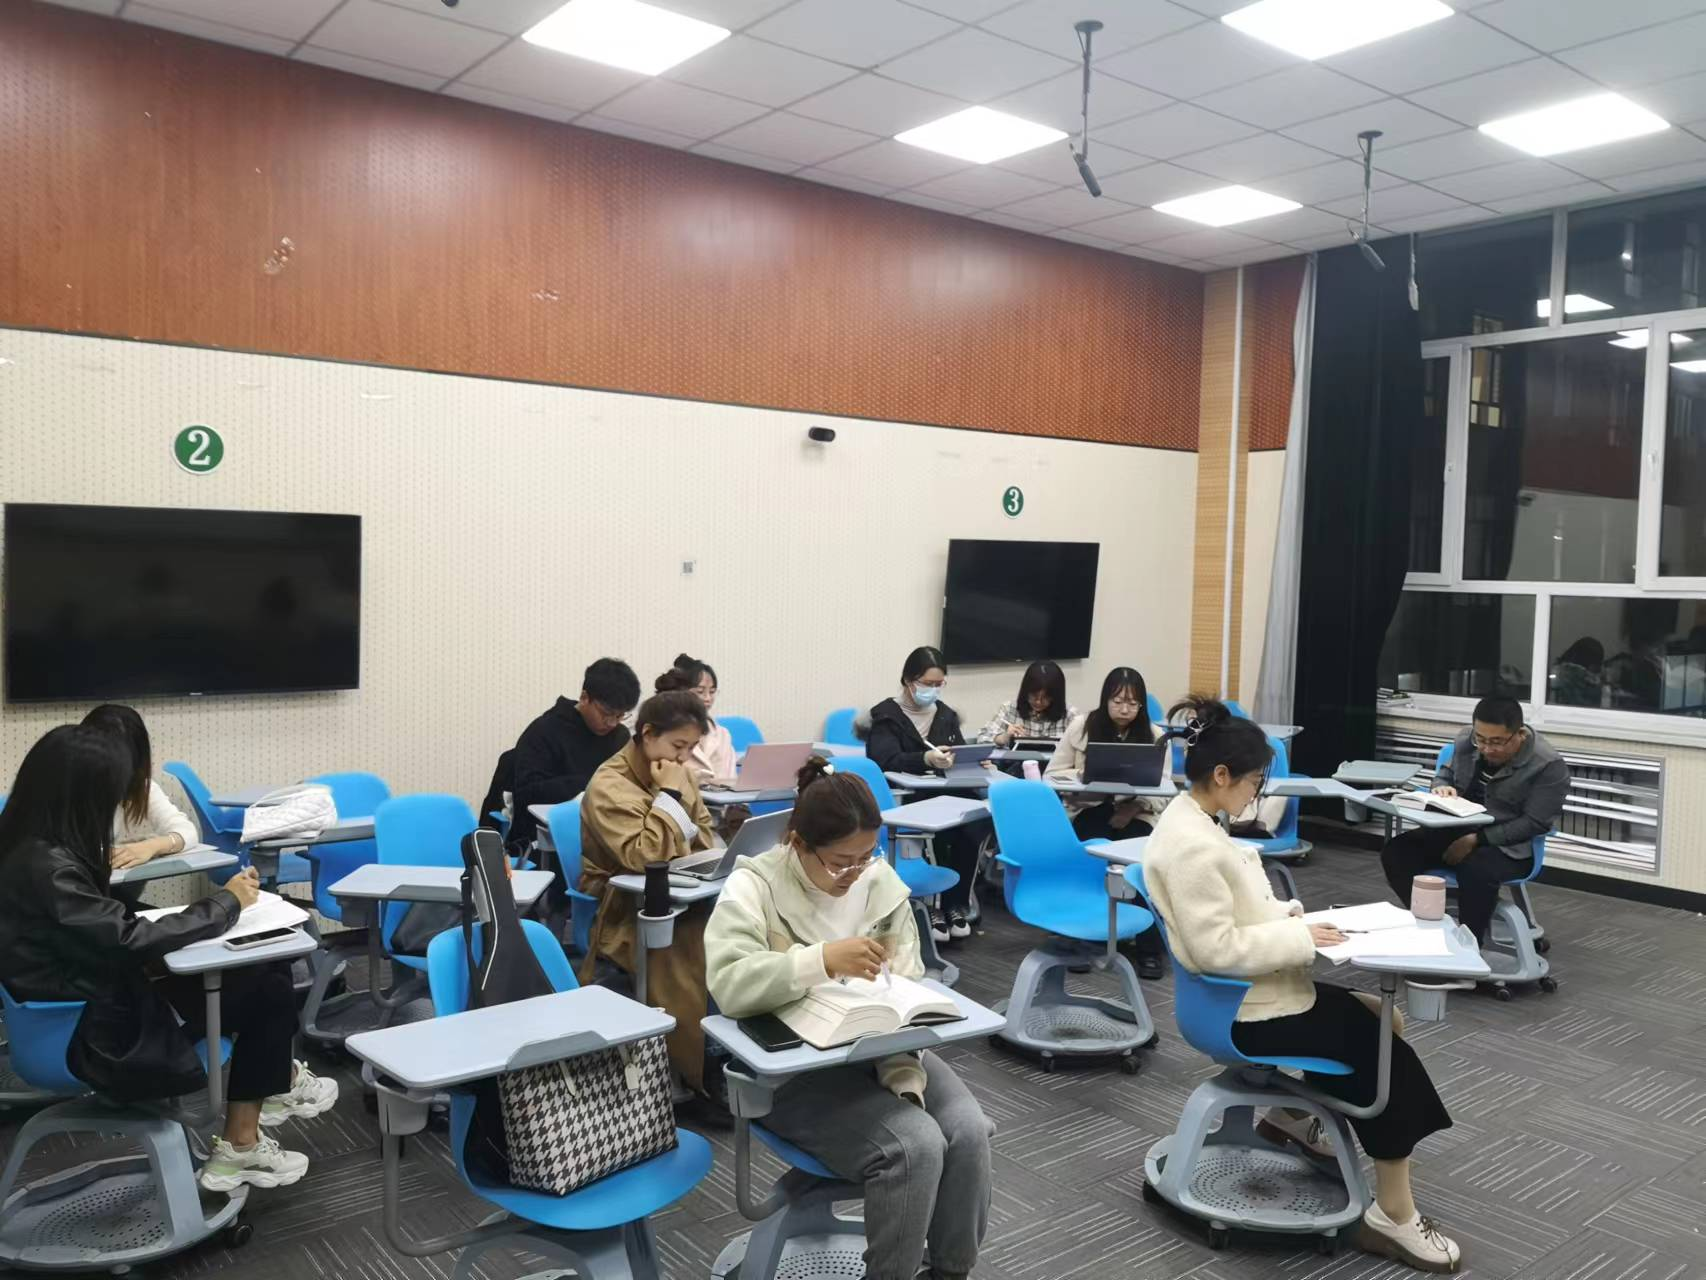
\includegraphics[width=1\linewidth]{10.23.jpg}
    \caption{第二期读书会实拍图(2023.10.23)}
    \label{fig1}
\end{figure}
2023年10月23日18:00—20:00,我们在东北林业大学奥林学院203教室开展了第二期的读书会。本期读书会我们阅读了《哲学的贫困》第二章第一节中的\textbf{“第五个说明”}与\textbf{“第六个说明”}。我们本期做了非常丰富的讨论,现场情况见\textbf{\nameref{fig1}}\footnote{在这里非常抱歉,由于本期读书会讨论的过于热情,以至于我在中途拍照的时候漏掉了一些同学与老师。},主要讨论内容可简要地概括如下:
\subsubsection{1.第五个说明}

在“第五个说明”中,马克思首先指出:
\begin{adjustwidth}{2em}{2em}
    \qquad\fangsong
    “如果把辩证运动的全部过程归结为简单地对比善和恶,归结为提出任务来消除恶并且把一个范畴用作另一个范畴的消毒剂,那末范畴就失去自己的独立运动;观念就“不再发生作用”;他就没有内在的生命。它既不能把自己安置为范畴,也不能把自己分解为范畴。范畴的顺序成了一种脚手架。辩证法已不是绝对理性的运动了。辩证法没有了,代替它的至多不过是最纯粹的道德而已。”
\end{adjustwidth}

这里马克思似乎是想表达:“辨证运动”并不是蒲鲁东所认为的那种“简单地对比善和恶,并提出任务来消除恶”。马克思认为蒲鲁东的“辩证运动”不过是借助他自己的搭建出的一种“脚手架”而进行的,这意味着蒲鲁东将黑格尔所认为的“范畴的自我运动”变成了通过他(指蒲鲁东)自己搭建起来的“脚手架”而进行的运动。因此,马克思会说,在蒲鲁东的“辩证运动”下,范畴本身“就没有内在的生命”了。

之后,马克思揭示了蒲鲁东自己的逻辑混乱。马克思认为,蒲鲁东在谈论“历史”的时候,他是从他自认为的“范畴的顺序”\footnote{根据前文的分析,不难理解,这种“范畴的顺序”是通过蒲鲁东自己构建的“脚手架”而展开的。}去出发的。但是,当蒲鲁东将他自认为的“范畴的顺序”应用到现实中时,便同现实产生了矛盾。因此马克思指出:
\begin{adjustwidth}{2em}{2em}
    \qquad\fangsong
    “……于是蒲鲁东先生只得承认,他用以说明经济范畴的次序和这些经济范畴在其中相互产生的次序是不相适应的。经济的进化不再是理性本身的进化了。”
\end{adjustwidth}

最后,马克思在“第五个说明”中的最后一部分的内容中强调,如果按照蒲鲁东所设想的“现实的历史是观念、范畴和原理在其中出现的那种历史顺序”的话,那末就必须对此进行进一步的追问。也即是说,如果说是某一时代的原理创造了这一时代的历史的话,那末,为什么这一时代的原理没有创造别的时代的历史呢?为什么这一时代的原理恰好地就出现在这一时代了呢?为了回答上述疑问,就必须进一步考察那一时代的人们是怎样进行生产生活的、那一时代的人们之间的关系是怎么样的。但只要进入到对具体时代的人们的生产生活的考察之中,那末就是背弃了那种认为“观念创造历史”的观点,就是回到了历史发生的真正出发点。

因此,马克思在最后是这么论述的:
\begin{adjustwidth}{2em}{2em}
    \qquad\fangsong
“我们暂且和蒲鲁东先生一同假定:现实的历史,适应时间次序的历史是观念、范畴和原理在其中出现的那种历史顺序。

每个原理都有其出现的世纪。例如,与权威原理相适应的是11世纪,与个人主义原理相适应的是18世纪,推其因果,我们应当说,不是原理属于世纪,而是世纪属于原理。换句话说,不是历史创造原理,而是原理创造历史。但是,如果为了顾全原理和历史我们再进一步自问一下,为什么该原理出现在11世纪或者18世纪,而不出现在其它某一世纪,我们就必然要仔细研究一下:11世纪的人们是怎样的,18世纪的人们是怎样的,在每个世纪中,人们的需求、生产力、生产方式以及生产中使用的原料是怎样的;最后,由这一切生存条件所产生的人与人之间的关系是怎样的。难道探讨这一切问题不就是研究每个世纪中人们的现实的、世俗的历史,不就是把这些人既当成剧作者又当成剧中人物吗?但是,只要你们把人们当成他们本身历史的剧中人物和剧作者,你们就是迂回曲折地回到真正的出发点,因为你们抛弃了最初作为出发点的永恒的原理。”
\end{adjustwidth}

\subsubsection{2.第六个说明}
马克思在这部分内容中开篇提到:
\begin{adjustwidth}{2em}{2em}
    \qquad\fangsong
    “我们已经看到,在这一切一成不变的、停滞不动的永恒下面没有历史可言,即使有,至多也只是观念中的历史,即反映在纯理性的辩证运动中的历史。蒲鲁东先生谈到辩证运动中的各种观念不能自相‘区分’时,把运动的一切影子和影子(它们可以造成某种类似历史的东西)的一切运动一概抹熬。”
\end{adjustwidth}

其中,\textbf{“运动的影子”}和\textbf{“影子的运动”}分别代表的是什么意思呢?在这里,我们认为前者指的是“感性历史”的理论表现,后者指的是黑格尔的那种“纯粹理性”的运动。因此,我们可以认为,马克思在这里想表明:蒲鲁东所谈论的“辨证运动”既不是对感性历史发展过程的理论表达,也不是对黑格尔式的纯粹理性的运动的表达。因此,正如前面我们所讨论的那样,事实上,蒲鲁东自己构建了一个范畴的“脚手架”,范畴遵循着蒲鲁东自己构建的“脚手架”向上爬行。而范畴为什么要踏着“脚手架”向上运动呢?因为蒲鲁东认为范畴就得踏着他所构建的“脚手架”向上运动,这似乎是蒲鲁东先生的一厢情愿。

既然蒲鲁东的“辨证运动”既不是对感性历史的理论表达,也不是对黑格尔式的“纯粹理性”运动的表达,那末,蒲鲁东是如何从底层逻辑层面说明他的“辩证运动”的合理性的呢?很简单,既然蒲鲁东自己的“辨证运动”既不是“运动的影子”也不是“影子的运动”,那末,蒲鲁东先生完全可以“大言不惭地”构建出一个新的规律,并用一种“唬人的词句”宣称这种规律的至高性地位。因此,蒲鲁东先生自己构建出了所谓的\textbf{“人类理性”}、\textbf{“社会天才”}等等的概念。然而事实上,我们不难看出,所谓的\textbf{“人类理性”}、\textbf{“社会天才”}等的概念不过是蒲鲁东自己虚构出来的东西,不过是蒲鲁东自己的主观设想。

因此,当蒲鲁东的理论同现实的历史之间发生矛盾的时候,他就将这些\textbf{“矛盾”}看作是\textbf{“人类理性”}、\textbf{“社会天才”}的任务,他认为\textbf{“人类理性”}、\textbf{“社会天才”}就是需要解决这些矛盾的,进而使得范畴朝着\textbf{“人类理性”}、\textbf{“社会天才”}所期待的目标发展。

因而我个人\footnote{指本书编者。}认为,在马克思的视角下,蒲鲁东的逻辑进路应可分为如下的步骤:


\begin{tcolorbox}[colback=gray!20, colframe=gray!100, sharp corners, leftrule={3pt}, rightrule={0pt}, toprule={0pt}, bottomrule={0pt}, left={2pt}, right={2pt}, top={3pt}, bottom={3pt}] 
\textbf{step1.}假定有一个“先在”的真理:例如“纯粹的平等”、“纯粹的自由”等最终的概念。

\textbf{step2.}假定一种“规则”:可以通过这种“规则”发现“真理”,并把这种“规则”命名为“人类理性”、“社会天才”。

\textbf{step3.}因此,当理论同现实相违背时,蒲鲁东就可以借着“人类理性”、“社会天才”的名义说:这种矛盾正是要通过“辩证运动”被解决的!


\end{tcolorbox}

因此,马克思会说:
\begin{adjustwidth}{2em}{2em}
    \qquad\fangsong
    “假设只是为了某种特定的目的而设立的。通过蒲鲁东先生之口讲话的社会天才首先给自己提出的目的,就是消除每个经济范畴的一切坏的东西,使它只保留好的东西。他认为,好的东西,最高的幸福,真正的实际目的就是平等。为什么社会天才只要平等,而不要不平等或友爱、不要天主教或别的什么原理呢?因为‘人类之所以实现这么多特殊的假设,正是由于考虑到一个最高的假设’,这个最高的假设就是平等。换句话说,因为平等是蒲鲁东先生的理想。他以为分工、信用、工厂,一句话,一切经济关系都仅仅是为了平等的利益才被发明的,但是结果它们往往对平等不利。由于历史和蒲鲁东先生的臆测步步发生矛盾,所以他得出结论说,有矛盾存在。即使是有矛盾存在,那也只存在于他的固定观念和现实运动之间。”
\end{adjustwidth}

在上面马克思的这段论述中,我们可以挑几句关键的句子来看,例如:\begin{fangsong}
    “通过蒲鲁东之口讲话的社会天才”
\end{fangsong},以及\begin{fangsong}
    “为什么社会天才只要平等,而不要不平等或友爱、不要天主教或别的什么原理呢?……因为平等是蒲鲁东先生的理想”
\end{fangsong}
等。不难看出,前面这几句话处处体现出了我在前文所概括的\textbf{“蒲鲁东的逻辑进路”}中的三个步骤。因此,马克思会指出:\begin{fangsong}
    “即使是有矛盾存在,那也只存在于他<指蒲鲁东>\footnote{编者注。}的固定观念和现实运动之间。”
\end{fangsong}

因此我们可以看到,马克思在这里最终想要表达的是:\textbf{蒲鲁东的思想既不唯物,也不客观。}在这里,我个人\footnote{指本书编者。}认为,蒲鲁东的思想既没有超越古典经济学家们,也没有超越黑格尔。因为,相较于古典经济学家们而言,蒲鲁东缺少了这些理论家们的唯物主义倾向;相较于黑格尔而言,蒲鲁东也没有领悟“辩证法”或“辨证运动”的实质,因而蒲鲁东的思想更像一种拙劣的“折衷主义”\footnote{事实上,我认为在“第七个说明”中马克思对蒲鲁东的这种“折衷主义”的批判会体现地更为明显,但本期讨论会并没有讨论到“第七个说明”,因此这里先按下不表。}。

在“第六个说明”的最后,马克思这样说道:
\begin{adjustwidth}{2em}{2em}
    \qquad\fangsong
    “当然,平等趋势是我们这个世纪所特有的。但是,说以往各世纪及其完全不同的需求、生产资料等等都是为实现平等而遵照天命行事,这首先就是把我们这个世纪的人和生产资料当做过去世纪的人和生产资料看待,否认世世代代不断改变前代所获得的成果的历史运动。经济学家们很清楚,同是一件东西对甲说来是成品,对乙说来只是从事另一种生产的原料。
    
    如果你们同蒲鲁东先生一道假定:社会天才制造出,或者更确切些说随兴制造出封建主,是为了达到把耕者变为负有义务的和彼此平等的劳动者这一天命的目的,那末,你们就是把目的和人换了一下,这种做法和为了达到恶意的满足(即羊群赶走人)而在苏格兰确立土地私有制的天命比较起来,毫不逊色。”
\end{adjustwidth}

马克思这两段论述同样地体现出了满满的历史唯物主义原则。马克思承认,“平等”确实是当时那个世纪所特有的思想倾向,但他想进一步表明的是,并不是自古以来就一直存在着这种“平等”的思想倾向的。如果将“平等”这种仅仅在当时那个世纪所特有的思想倾向看作是永恒不变的思想倾向的话,就意味着,当时那个世纪的人的物质生产活动同以往一切世纪的物质生产活动之间并无差别了。而这种观念是反历史唯物主义的,在这里就不赘述了。

\subsubsection{本期小结:以及一些余论}
本期我们讨论的比较热烈,同时一些新同学也在本期加入了我们的讨论会。在本期讨论会的最后几分钟,我们初步探讨了一下古典国民经济学(特别是李嘉图的经济学)同马克思主义经济学之间的差异。我们探讨了“李嘉图难题”的产生,以及马克思是如何解决李嘉图难题的(但我们只是初步地提了一嘴,并没有深入讨论下去)。我们计划在下期的讨论会中留一段时间和大家讨论一下李嘉图的利润理论与马克思之间的差异,以及马克思是如何系统地批判李嘉图经济学的。总之,这是一期收获很满的讨论会。
\newpage
\section{第三期:《哲学的贫困》选读(完结)+《雇佣劳动与资本》(1)}

\subsection{读书会记录}
2023年11月6日18:00—20:00,我们在东北林业大学奥林学院203教室开展了第三期的读书会\footnote{编者注:由于2023年10月30日大家感冒的比较多,我们就将第三期读书会推迟到了11月6日。}。本期读书会我们结束了《哲学的贫困》第二章第一节的讨论,由于前两期的积累,我们对于《哲学的贫困》第二章第一节中\textbf{“第七即最后一个说明”}这部分内容的讨论比较顺利。之后,我们开启了马克思的另一篇政治经济学经典著作《雇佣劳动与资本》的讨论。总之,和之前几期一样,我们进行了充分而深刻的讨论,具体内容可概括如下:

\subsubsection{1.第七即最后一个说明}
“第七个说明”这部分内容更像是对前面六个说明的总结,整体读下来不难理解,不过还是存在一些值得深入讨论的细节之处。
例如,马克思的这两段话是这么说的:

\begin{adjustwidth}{2em}{2em}
    \qquad\fangsong
 “这样,为了正确地判断封建的生产,必须把它当做以对抗为基础的生产方式来考察。必须指出,财富怎样在这种对抗中间形成,生产力怎样和阶级对抗同时发展,这些阶级中一个代表着社会上坏的、否定的方面的阶级怎样不断地成长,直到它求得解放的物质条件最后成熟。这难道不是说,生产方式、生产力在其中发展的那些关系并不是永恒的规律,而是同人们及其生产力发展的一定水平相适应的东西,人们生产力的一切变化必然引起他们的生产关系的变化吗?由于最重要的是不使文明的果实(已经获得的生产力)被剥夺,所以必须粉碎生产力在其中产生的那些传统形式。从此以后,从前的革命阶级将成为保守阶级。

资产阶级开始自己的历史发展时就有一个本身是封建时期无产阶级残存物的无产阶级存在。资产阶级在其历史发展过程中不可避免地要发展它的对抗性质,起初这种性质或多或少是掩饰起来的,只是处于隐蔽状态。随着资产阶级的发展,在它的内部发展着一个新的无产阶级,即现代无产阶级。无产阶级同资产阶级之间展开了斗争,在双方尚未感觉、注意、重视、理解、承认并公开宣告以前,这个斗争最初仅表现为局部的暂时的冲突,表现为一些破坏行为。另一方面,如果说现代资产阶级的全体成员由于组成一个与另一个阶级相对立的阶级而有共同的利益,那末,由于他们互相对立,他们的利益又是对立的,对抗的。这种利益上的对立是由他们的资产阶级生活的经济条件产生的。资产阶级运动在其中进行的那些生产关系的性质绝不是一致的单纯的,而是两重的;在产生财富的那些关系中也产生贫困;在发展生产力的那些关系中也发展一种产生压迫的力量;只有在不断消灭资产阶级个别成员的财富和形成不断壮大的无产阶级的条件下,这些关系才能产生资产者的财富,即资产阶级的财富;这一切都一天比一天明显了。”
\end{adjustwidth}

这里马克思主要是在阐述他的历史唯物主义思想。我们可以看到,在上面的第一段中,马克思说:
\begin{adjustwidth}{2em}{2em}
    \qquad\fangsong
    “这难道不是说,生产方式、生产力在其中发展的那些关系并不是永恒的规律,而是同人们及其生产力发展的一定水平相适应的东西,人们生产力的一切变化必然引起他们的生产关系的变化吗? ”
\end{adjustwidth}

在这里便有一个疑问,什么叫\textbf{“生产方式在其中发展的那些关系”}呢?我们知道,在马克思看来,“生产方式”本身就应包涵着“生产关系”与“生产力”两个维度,但马克思在这里又说“生产方式在其中发展的关系”,这是否有同义反复的嫌疑了呢?我们认为,这是一种很微妙的说法,马克思在这里想表示的应该就是“生产关系”本身,或者认为,马克思这里说的“生产方式”是一种更为具体的“生产形式”,也是生产力的一种表现。总之,这并不影响整段所论述的思想,这一细节之处可留给读者们细细思索。

此外,在上面的第二段中,马克思论述了无产阶级的生成以及无产阶级同资产阶级二者的斗争。马克思在这里对无产阶级的描述同样比较微妙,马克思既不是从经济关系出发,将无产阶级表述为不占有生产资料的阶级,也不是从哲学层面出发,即像在《<黑格尔法哲学批判>导言》中所表述的那样:“一个被戴上彻底的锁链的阶级,一个并非市民社会阶级的市民社会阶级,形成一个表明一切等级解体的等级”\footnote{编者注:见马克思《<黑格尔法哲学批判>导言》}。

我们认为,马克思在这里更想说明的是无产阶级的自我发展过程,即从自在到自为的过程。马克思在这里首先指明了无产阶级最早生成于资本主义发展的初期,从某种意义上说,无产阶级是伴随着资产阶级的发展而发展的。然而在资本主义发展的前期,无产阶级与资产阶级之间的阶级对抗不明显,因而在那一时期,资本主义社会的对抗性质“或多或少是掩饰起来的,只是处于隐蔽状态。”因此,在这种对抗性不明显的社会下,无产阶级的阶级意识\footnote{编者注:这里借用了卢卡奇的术语“阶级意识”。}同样是不明显的,这便是一种“自在”的状态。而随着资本主义社会的进一步发展,阶级对抗也愈来愈明显,如马克思所言,资产阶级的运动由于资本主义生关系的作用所表现出了双重性的结果,即资产阶级的历史运动一方面制造着大量的财富(但这种财富是个别性的、属于个别资产阶级成员的财富),另一方面同时又制造着大量的贫困(这种贫困是一种普遍性的贫困)。这种直接在物质利益上的对抗促使了无产阶级的阶级意识的提高,也意味着无产阶级从“自在”向“自为”的转变\footnote{编者注:这里用的词是“转变”,并没有明确指出无产阶级必然会随着物质利益的对抗而成为“自为阶级”,因为其实在这里有一些疑问,当代资本主义国家的工人阶级是否可以被称作是“自为阶级”呢?}。

马克思在“第七个说明”后面部分的论述就很像《共产党宣言》了。不过马克思在《共产党宣言》中是对形形色色的社会主义者进行了划分,而在“第七个说明”中则是对政治经济学语境下的形形色色的改良主义学派进行了划分。在这里,按照马克思在“第七个说明”中的划分,我给大家做一个简短的归纳总结:
\begin{tcolorbox}
    \textbf{1.宿命论的经济学家:}斯密、李嘉图等代表的古典政治经济学,可以被看作是一种无批判的实证主义。

    \textbf{2.浪漫派:}对宿命论经济学家的直接继承,但他们甚至认为无产阶级的贫困是“理所应当”的。

    \textbf{3.人道学派:}企图在道德层面约束资产阶级。

    \textbf{4.博爱学派:}人道学派的进一步完善,幻想着人人都能变成资产者。

    \textbf{5.空想社会主义者:}在无产阶级解放的物质存在条件不足的情况下,企图寻得无产阶级解放的理论。
\end{tcolorbox}

最后,回到出发点,马克思对蒲鲁东做了一个总结性的评论,在这里我们就不过多解释了,我仅把原文放出来,根据前面几期的内容读者们应该能够体会到马克思的意思了。

马克思在最后写道:
\begin{adjustwidth}{2em}{2em}
    \qquad\fangsong
    “现在再来谈谈蒲鲁东先生。

每一种经济关系都有其好的一面和坏的一面;只有在这一点上蒲鲁东先生没有背叛自己。他认为好的方面由经济学家来揭示,坏的方面由社会主义者来揭发。他从经济学家那里借用了永恒经济关系的必然性这一看法;从社会主义者那里借用了使他们在贫困中只看到贫困的那种幻想。他对两者都表示赞成,企图拿科学权威当靠山。而科学在他的观念里已成为某种微不足道的科学公式了;他无休止地追逐公式。正因为如此,蒲鲁东先生自以为他既批判了政治经济学,也批判了共产主义;其实他远在这两者之下。说他在经济学家之下,因为他作为一个哲学家,自以为有了神秘的公式就用不着深入纯经济的细节;说他在社会主义者之下,因为他既缺乏勇气,也没有远见,不能超出(哪怕是思辨地也好)资产者的眼界。

他希望成为一种合题,结果只不过是一种总合的错误。

他希望充当科学泰斗,凌驾于资产者和无产者之上,结果只是一个小资产者,经常在资本和劳动、政治经济学和共产主义之间摇来摆去。”
\end{adjustwidth}

\subsubsection{2.雇佣劳动与资本(1)}
本期讨论会我们把《雇佣劳动与资本》开了个头,本期具体讨论的内容在我们所编排的讲义的18—21页。在进一步展开我们的讨论内容之前,我有必要跟读者们交代一下《雇佣劳动与资本》这部著作的写作背景以及后续恩格斯在1891对此做出的一些修改与补充。

\paragraph{一个简要的背景概述}\begin{fangsong}
《雇佣劳动与资本》这部著作是马克思根据1847年12月在布鲁塞尔德意志工人协会发表的演说写成的,最初以社论形式于 1849年4月5—8日和11日在《新莱茵报》陆续发表。后来由于《新莱茵报》被迫停刊,这部著作的连载遂告中断。 
时间来到1891年,为适应工人群众学习科学社会主义理论的需要,在恩格斯的关心下,这部著作的新单行本在柏林印行。 恩格斯根据《资本论》的基本观点和科学论述,对马克思这部著作进行了适当的修改和补充,并为该著作的单行本写了一篇《导言》。 恩格斯在《导言》中指出:“我所作的全部修改,都归结为一点。 在原稿上是,工人为取得工资向资本家出卖自己的劳动,在现在这一版本中则是出卖自己的劳动力。”\footnote{编者注:见马恩选集第一卷(中央编译局2012年版)第318页。}恩格斯阐明了修改的理由,论述了马克思主义政治经济学的科学价值,揭露了资本主义制度的本质,指出工人阶级不仅是社会财富的生产者,而且是新的社会制度的创造者。
\end{fangsong}

事实上,就马克思在1849年在《新莱茵报》发表的原版内容而言,我们不得不承认其中存在着不可忽视的局限性,当时的马克思并没有完成他的政治经济学批判工作,虽然当时他能够在整体性层面洞察出资本主义经济社会的固有局限,但是就一些关键的细节之处,例如对“劳动”与“劳动力”之间的区分,马克思的观点还是处于一个模糊的状态。然而经过恩格斯修改之后的版本就好多了。

 \vspace{0.5cm} %设置垂直距
\textbf{在把背景交代清楚之后,接下来便可以展开我们的讨论了。}
首先,按照原文的顺序,我们跟着马克思的思路讨论了“什么是工资?”的问题。对于这一问题的回答我们首先需要从现实的经验现象中去寻找答案。马克思说,假如去问工人们什么是他们的工资,他们会回答:“工资是工作的一定时间所换来的报酬。”可见,工资似乎表现为是工人同资本家之间进行的交换所获得的价值物,更确切地说,似乎是工人工作的一定时间(或一定量的工作)同资本家之间进行的交换所获得的价值物。但事实上并非如此,因为当我们考虑一下这个“交换”本身是否同其他商品之间的交换存在着差异时,我们便会发现,工人为获取工资同资本家之间进行的交换同他为获取生活资料同卖主进行的交换没有什么不同:这种交换总是遵循着“等价交换”的原则的\footnote{编者注:因为如果不是这样的话,商品经济本身便会出现混乱。}。那为什么工人所获得的工资与工人所生产出的商品的价值量之间存在着不一致呢?事实上,问题的关键则在于,工人同资本家所付给他的工资之间所进行的等价交换的那个“物”并不是劳动本身,而是劳动力商品。事实上,劳动是无法成为商品的,劳动本身没有价值,关于这一点的详细论述,大家可以去看《资本论》第一卷第四章的“劳动力的买和卖”以及第六章的“工资”\footnote{编者注:事实上,在《雇佣劳动与资本》中,即使是恩格斯修改之后的版本,也并没有详细地论述劳动力商品同劳动之间的差异性,因为恩格斯是直接根据《资本论》第一卷对其进行的修改与增补的,因而在其中有些概念的出场会显得缺少一些前提性的阐述,因此,我还是推荐大家直接去看《资本论》第一卷,这是一个苦功夫,需要静下心来好好研读,在这里我就不赘述其具体内容了。}。

\textbf{因此,仅仅就劳动力商品与工资之间的交换而言,这一过程不存在剥削!}\footnote{编者注:请读者们记住这一点,在不考虑生产价格理论的前提下,这一点是完全正确的,我和光玉、许婕老师都是赞成的,但是在后面关于劳动与自由之间的关系时,我们之间发生了一定的分歧。}如果有人固执地认为劳动力商品同工资之间的交换过程发生了剥削,我想他大概率是不懂马克思主义政治经济学的。

接下来的这一段引起了我们的广泛讨论:

\begin{adjustwidth}{2em}{2em}
    \qquad\fangsong
“可是,劳动是工人本身的生命活动,是工人本身的生命的表现。工人正是把这种生命活动出卖给别人,以获得自己所必需的生活资料。可见,工人的生命活动对于他不过是使他能以生存的一种手段而已。他是为生活而工作的。他甚至不认为劳动是自己生活的一部分;相反地,对于他来说,劳动就是牺牲自己的生活。劳动是已由他出卖给别人的一种商品。因此,他的活动的产物也就不是他的活动的目的。工人为自己生产的不是他织成的绸缎,不是他从金矿里开采出的黄金,也不是他盖起的高楼大厦。他为自己生产的是工资,而绸缎、黄金、高楼大厦对于他都变成一定数量的生活资料,也许是变成棉布上衣,变成铜币,变成某处地窖的住所了。一个工人在一昼夜中有十二小时在织布、纺纱、钻孔、研磨、建筑、挖掘、打石子、搬运重物等等,他能不能认为这十二小时的织布、纺纱、钻孔、研磨、建筑、挖掘、打石子是他的生活的表现,是他的生活呢?恰恰相反,对于他来说,在这种活动停止以后,当他坐在饭桌旁,站在酒店柜台前,睡在床上的时候,生活才算开始。在他看来,十二小时劳动的意义并不在于织布、纺纱、钻孔等等,而在于这是挣钱的方法,挣钱使他能吃饭、喝酒、睡觉。假如说蚕儿吐丝作茧是为了维持自己的生存,那末它就可算是一个真正的雇佣工人了。”
\end{adjustwidth}

马克思在这里说:“可见,工人的生命活动对于他不过是使他能以生存的一种手段而已。他是为生活而工作的。他甚至不认为劳动是自己生活的一部分;相反地,对于他来说,劳动就是牺牲自己的生活。”
关于这一方面的论述,可以引申到对\textbf{劳动与自由之间的关系}的讨论。\textbf{在关于这一点的看法上,我们出现了分歧。}下面我将尽我所能还原当时我们争论的情况\footnote{编者注:遗憾的是,正如马克思的好朋友、著名的诗人海涅曾在其所著的《论德国宗教和哲学的历史》一书中所言的那样:“箭一离开弦便不再属于射手了,言论一离开说话人的口……便不再属于他了。”即使我全程极度认真地参与了这场讨论,但我也无法完全准确地描绘当事人的思想观点,请原谅我可能在某些地方对当事人的观点存在着的误解。}:

\paragraph{观点1:}\begin{fangsong}
以往似乎有一种误解,认为自由王国只有在共产主义社会才能达到,但其实在资本主义社会,自由王国与必然王国二者是以一种二分的形式所存在着的。诚然,当工人将自己的劳动力商品出卖给资本家之后,在资本家使用劳动力商品进行价值生产的这一过程中,工人事实上是不自由的,是处在一种“必然王国”之中。但是,一旦工人脱离生产过程,也即是说,当工人跨入到对于其自身的劳动力商品的恢复过程之中时,他实际上是暂时性地脱离了必然王国,进入到自由王国之中了。这应该如何理解呢?可以认为对于“工人恢复其自身劳动力商品”的这一过程而言,这一过程不涉及生产的领域,换句话说,这一过程仅仅是工人的纯粹消费的领域,不涉及价值与剩余价值的创造。因而这一领域不具有任何剥削性,换言之,这一领域是工人真正的生活领域——对于工人而言的仅仅纯粹的消耗使用价值的领域,完全是一个自然的过程。举个例子,比如说某工人一天工作了八个小时,赚了100块钱,他下班了给自己买了一个烤鸭吃,从这一行为中是无法分析出什么样的社会关系的,这一行为仅仅是工人消耗使用价值的过程,因而从这个意义上来说,这一个过程是“自由”的(至少相对于生产过程而言是自由的)。
\end{fangsong}
\paragraph{观点2:}\begin{fangsong}
我们认为“观点1”中所认为的那种“工人的纯消费领域属于自由王国”的看法是存在局限性的。我们同样承认剩余价值产生于生产领域,这即意味着在工人的纯消费领域不存在着剥削。但我们认为对于问题的分析不能止步于此。因为事实上,工人的消费可以被看作是资本主义生产过程的延申。诚然,工人在纯消费领域进行的活动仅仅是对使用价值的消耗,但这并不意味着工人阶级脱离了必然王国,我们认为工人阶级仍然是非自由的。这是因为,工人阶级的消费事实上具有两重性:一方面满足了工人阶级自身的物质需求\footnote{编者注:我们甚至对这种“满足工人阶级自身物质需求”的观点还是持有保留意见的,因为处于贫困水平的工人阶级似乎连这一点也无法被满足。};另一方面,工人阶级的消费事实上为资本主义的再生产创造了条件,而这一方面则是我们批判“观点1”的关键。我们认为,工人阶级的消费实际上处于一种“知其不可而为之”的境遇,工人阶级为了生存(生活)他必须进行消费,但工人阶级的这种消费同时又为下一次资产阶级对其的剥削创造了物质条件。在这里我们做一个简单的政治经济学分析:对于资本家而言,雇佣工人进行生产这一过程诚然是至关重要的,因为这一过程直接涉及到了价值与剩余价值的生成、涉及到了资本家对工人阶级的剥削,但是生产过程的结束对于资本家而言并不是直接的结果,资本家必须要使得剩余价值转换为最终的利润\footnote{编者注:这涉及到马克思的生产价格理论,在这里就不赘述了。有兴趣的读者可以阅读《资本论》第三卷的前10章。},而这种转换恰恰是通过工人阶级的消费而得以实现的。因此,在这个意义上,我们认为工人阶级的纯消费领域依然是受到着资本主义制度的规制,并没有脱离必然王国。    
\end{fangsong}
\vspace{0.5cm} %设置垂直距

我们之间的分歧主要是“观点1”和“观点2”之间的分歧。光玉老师的看法倾向于“观点1”,我和许婕老师的看法倾向于“观点2”。并且,从某种意义上而言,我们似乎都能够理解彼此观点的侧重之处。事实上,我认为,在政治经济学原理部分,我们都能清晰地认识到剩余价值的生产与剩余价值的实现之间的区别,我们也都能理解商品经济的等价交换原则。因此,相较于政治经济学原理而言,我们之间更像是对于“自由”这一范畴的看法出现了分歧,而对于“自由”的理解,在我看来是一个哲学问题,因而我们之间的分歧,确切的说是一个哲学层面的分歧。

事实上,马克思早年就在其博士论文《论德谟克利特的自然哲学与伊壁鸠鲁的自然哲学之差别》中探讨了“自由”的问题。当时的马克思由于受到青年黑格尔派的自我意识哲学的影响,他致力于通过诉诸一种“抽象个别性的自我意识”的形式去对抗当时存在着的普遍的宗教威权。(关于这部分的内容,我就不在这里赘述了,有兴趣的读者可以自行去阅读马克思的博士论文,或者在将来的读书会中继续探讨这部分的内容\footnote{编者注:估计这学期不会讨论到这部分内容了,这学期的主题是马克思的政治经济学。}。)当然,现在我们知道,当时的马克思的自由思想是存在着局限性的,因为对于“抽象个别性的自我意识”的形式而言,其代表的是一种“脱离定在的自由”,马克思甚至在当时也意识到了这种“自由”是无法“在定在之光中发亮”的。

让我们顺着这个思路继续下去,我们会意识到,不存在绝对的自由。进而再次回到我们之间争论的出发点,“工人阶级的纯消费领域”的自由\footnote{编者注:我们暂且假定这种自由存在。}便是一种“定在”之中的自由,而这个“定在”本身就是资本主义社会,更具体地说,是资本主义市场机制。我想关于我在上面的那种诠释,我们之间应该都是认同的。如果大家都能够接受这一点的话,那末争论的焦点便又一次地被转移了,现在的问题变成了\textbf{工人阶级在资本主义市场经济下的“消费自由”是否是“真实的自由”?}关于这一问题,我想我在这里还是不要做出回答的好,这部分留给读者们细细思索了。

\subsubsection{本期小结:以及一些余论}
本期讨论会的人数比较少,但却是讨论的最为热烈的一期。当天哈尔滨下了一天的大雪,不过恶劣的天气却丝毫没有减少大家学习与讨论的热情,我想这就是马克思主义政治经济学的魅力吧!此外,在本期讨论会中,我们还提到了20世纪60年代出现的“斯拉法体系”、马克思的“地租理论”、恩格斯对农民问题的研究、日本马克思经济学家置盐信雄提出的“置盐定理”、森岛通夫提出的“马克思基本定理(FMT)”等。这些内容大多是在讨论某一具体点的时候顺便提的一嘴,没有具体的深入展开。事实上,上述提到的每个部分都蕴含着极为丰富的内容,限于篇幅限制,我就不把这些具体内容编排到本书中了,如果有成员对某一方面感兴趣的话,可以在群里提出来,我会给大家发相关的学习资料。总而言之,这是一期收获满满的讨论会。






\end{document}
